\chapter{CSS}

\section{What is CSS}

Cascading Style Sheets (CSS) is a language for specifying how documents are presented to users.

A document is a collection of information that is structured using a markup language.

Presenting a document to a user means converting it into a useable form for your audience.

\begin{HTML5}[demo]
<!DOCTYPE html>
<html>
  <head>
  <meta charset="UTF-8">
  <title>Sample document</title>
  </head>

  <body>
    <p>
      <strong>C</strong>ascading
      <strong>S</strong>tyle
      <strong>S</strong>heets
    </p>
  </body>
</html>
\end{HTML5}

\section{Why use CSS}

Keeping the styles separate from your HTML content:
\begin{itemize}
\item Helps avoid duplication
\item Makes maintenance easier
\item Allows you to make a site-wide change in one place
\end{itemize}


\begin{CSS}[style1.css]
strong {color:red;}
\end{CSS}

\begin{HTML5}
<!DOCTYPE html>
<html>
  <head>
  <meta charset="UTF-8">
  <title>Sample document</title>
  <link rel="stylesheet" type="text/css" href="style1.css">
  </head>

  <body>
    <p>
      <strong>C</strong>ascading
      <strong>S</strong>tyle
      <strong>S</strong>heets
    </p>
  </body>
</html>
\end{HTML5}

\section{How CSS works}

\begin{itemize}
\item The browser converts the markup language and the CSS into the DOM (Document Object Model). The DOM represents the document in the computer's memory. It combines the document's content with its style.
\item The browser displays the contents of the DOM.
\end{itemize}


\section{CSS Rule}

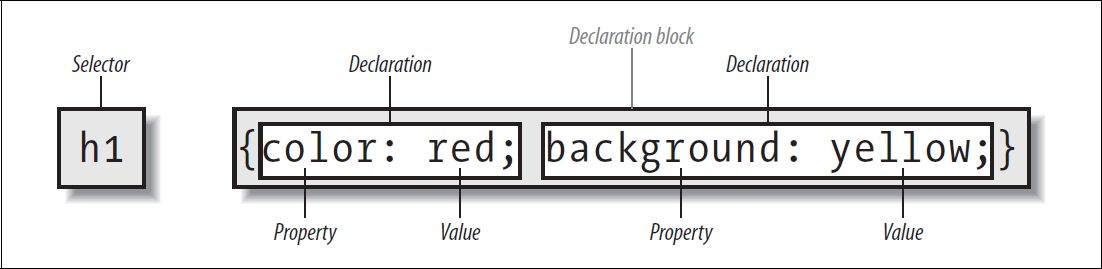
\includegraphics[scale=0.75]{css/resources/css-rule.jpg}

\section{Selector}

A selector is a chain of one or more sequences of simple selectors separated by combinators.

A sequence of simple selectors is a chain of simple selectors that are not separated by a combinator.



选择器是通过combinator分割开的一系列选择器组合起来的。

而一系列选择器是一系列简单选择器他们之间没有被combinator分开。

简单选择器是一个type selector, universal selector, attribute selector, class selector, ID selector, content selector, pseudo class。 而一个pesudo element可能出现在简单选择器的最后(???这个时候是简单选择器,还是一系列选择器??)。


\subsection{Simple selector}

A simple selector is either a type selector, universal selector, attribute selector, class selector, ID selector, content selector, or pseudo-class. One pseudo-element may be appended to the last sequence of simple selectors.

\subsubsection{Type selector}

A type selector is the name of a document language element type.

就是HTML的标签名来选择元素。

\begin{CSS}
<style>
p {color:red;}
div {border:1px; border-style:solid;}
</style>

<p>first line</p>
<p>second line</p>
<div>third line</div>
\end{CSS}


\subsubsection{Universal Selector}



\subsection{规则应用}

如果有多条规则应用到同一个元素,那么哪条规则会最终取胜。CSS提供了三种机制:继承,层叠和特指。


\subsubsection{继承}

从祖先元素继承样式;CSS中很多属性是可以继承的,相当一部分和文本相关,如颜色,字体,字号。

也有很多属性是不能继承的(因为继承这些属性没有意义)。不能继承的主要是涉及到元素盒子的定位和显示方式。比如边框,外边距,内边距。

\subsubsection{层叠}

对于元素中某个标签的特定属性值有多个来源是,最终确定使用哪个值。

Style sheets may have three different origins: author, user, and user agent.

样式来源主要有三个,浏览器,用户和作者:
\begin{itemize}
\item 第一,首先浏览器有个默认的样式表;
\item 然后,有一个用户样式表,可以通过用户样式表,来强制所有网站按这个样式来显示;
\item 在这就是作者样式表,有三种方式:连接样式,嵌入样式和行内样式
\end{itemize}

层叠顺序
\begin{enumerate}
\item 浏览器默认样式表
\item 用户样式表
\item 作者连接样式表(按照特闷连接到页面的先后顺序)
\item 作者嵌入样式
\item 作者行内样式
\end{enumerate}

按上面的顺序来更新对每个标签属性的值,这个检查结束后,再将每个标签以最终设定的样式显示出来。

The CSS cascade assigns a weight to each style rule. When several rules apply, the one with the greatest weight takes precedence. 

By default, rules in author style sheets have more weight than rules in user style sheets. Precedence is reversed, however, for "!important" rules. All user and author rules have more weight than rules in the UA's default style sheet. 


最终的层叠规则是:
\begin{enumerate}
\item 先找出每个元素以及元素的属性;
\item 按照顺序和权重排序,顺序就是上述五个来源来选择,权重可以通过\lstinline$空格!important$来加重声明的权重。
\item 按特指读排序。表示一条规则有多明确,则优先级别高
特制度计算:I-C-E
\begin{itemize}
\item 选择符中有一个ID,就在I的位置上加1;
\item 选择符中有一个类,就在C的位置上加1;
\item 选择符上有一个元素标签名,就在E的位置加上1;
\end{itemize}
\item 如果所有都一样,则声明靠后的优先级别高
\end{enumerate}




\subsection{CSS Specification}

Once a user agent has parsed a document and constructed a document tree, it must assign, for every element in the tree, a value to every property that applies to the target media type.

The final value of a property is the result of a four-step calculation: the value is determined through specification (the "specified value"), then resolved into a value that is used for inheritance (the "computed value"), then converted into an absolute value if necessary (the "used value"), and finally transformed according to the limitations of the local environment (the "actual value").

%\paragraph{Specified Value}
\begin{itemize}
\item If the cascade results in a value, use it.
\item Otherwise, if the property is inherited and the element is not the root of the document tree, use the computed value of the parent element. 
\item Otherwise use the property's initial value. The initial value of each property is indicated in the property's definition. 
\end{itemize}

%\paragraph{Compute Value}

%\paragraph{Used Value}

%\paragraph{Actual Value}



\section{属性}

\subsection{Property Definition}



属性值主要分为三类:

\begin{itemize}
\item 文本值
\item 数字值,数字值分为绝对值和相对值;

绝对值这里我们只使用像素(px);

相对值有(em, ex, \%),em表示一种字体中字母"M"的宽度,ex等于字体中字母"x"高度。\%百分比适合设定诶包含的元素的宽度。

\item 颜色值,颜色名(red),16进制颜色(\#RGB,\#RRGGBB),RGB颜色值(rgb(0,255,0)),RGB百分比值(R\%,G\%,B\%),HSL(色相,饱和度\%,亮度\%)
\end{itemize}


\section{定位元素}

盒模型就是页面中的每个元素生成的矩形盒子。这些合资都要按照课件板式模型在页面上排布。主要由三个属性控制:position,display,float。

其中,position属性控制页面上元素间的位置关系;display控制元素是堆叠,还是并排,还是根本不在页面上出现;float属性提供控制的方式,以便把元素组成多栏布局(???这个解释不是太清楚)。

\subsection{盒模型}

盒子的属性:
\begin{itemize}
\item 边框(border),可以设置边框的宽窄,样式和颜色;
\item 内边距(padding),可以设置盒子内容区域边框的间距;
\item 外边距(margin),可以设置盒子与相邻元素的间距。
\end{itemize}

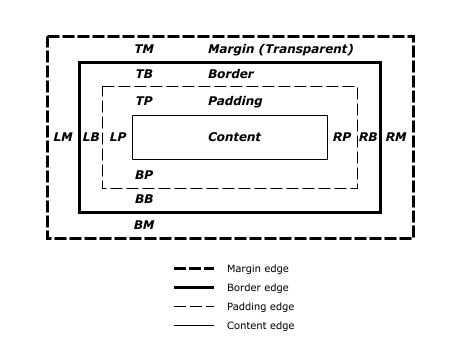
\includegraphics[scale=1]{css/resources/box-mode.png}


\begin{CSS}[上 右 下 左]
{margin: 5px 10px 12px 18px;}
\end{CSS}

如果有值没有写,则取对边的值,如果只写了一个值,则四边都取这个值。


border三个属性 宽度(width), 样式(style), 颜色(color)。 border还有第四个属性radius,但是不影响和模型的定位。

\begin{CSS}[三个粒度]
{border: 2px dashed red;} // 全部3个属性,全部4条边
{border-style: dashed;} // 一个属性,四条边
{broder-left-style: dashed;} // 一个属性,一条边
\end{CSS}

内边框和外边框。


\begin{CSS}[中和外边框和内边框,使不同浏览器效果一致]
* {margin: 0; padding: 0;}
\end{CSS}


(!!!!我记得这和有个什么显示方式有关,默认情况下上下排列才是垂直方向上外边距叠加,需要看文档补充一下)
垂直方向上的外边距会叠加。

外边框叠加,比如有两个段落,第1个段落的下外边距是50px,第2个段落的上外边框为30px,那么他们之间的外边框是50px。因为这种上下外边框相遇的情况下,他们会相互重叠,直到一个外边框碰到另一个元素的边框。

\subsubsection{盒子大小}

对于块级元素,如果没有设置width,那么他的默认值就是auto,结果会让元素的狂度扩充到与父元素同宽;如果添加水平边框,内边距和外边距,会导致内容宽度减少,减少量等于水平边框,内边距和外边距增加之和。

明确设定width之后,块级元素就不会再扩展到与父元素同宽了。盒子width属性指定的只是盒子内容区的宽度,而不是盒子要占住的水平宽度。


\subsection{float \& clear}

